\documentclass[a4paper,11pt]{exam}
%\printanswers % pour imprimer les réponses (corrigé)
\noprintanswers % Pour ne pas imprimer les réponses (énoncé)
\addpoints % Pour compter les points
% \noaddpoints % pour ne pas compter les points
%\qformat{\textbf{\thequestion ) } }
\qformat{\textbf{\thequestion )} \textit{(\thepoints)} \\  } % Pour définir le style des questions (facultatif)
\usepackage{color} % définit une nouvelle couleur
\shadedsolutions % définit le style des réponses
% \framedsolutions % définit le style des réponses
\definecolor{SolutionColor}{rgb}{0.8,0.9,1} % bleu ciel
\renewcommand{\solutiontitle}{\noindent\textbf{Solution:}\par\noindent} % Définit le titre des solutions

\usepackage{multicol}
\usepackage{caption}
\usepackage{tikz}
\usepackage{tkz-tab}
\usepackage{array}
\usetikzlibrary{trees}
\usepackage[final]{pdfpages}


\makeatletter

\def\maketitle{{\centering%
	\par{\huge\textbf{\@title}}%
	\par{\@date}%
	\par}}

\makeatother

\lhead{NOM Pr\'enom :}
\rhead{\textbf{Les r\'eponses doivent \^etre justifi\'ees}}
\cfoot{\thepage / \pageref{LastPage}}


%\usepackage{../../pas-math}
%\usepackage{../../moncours}


%\usepackage{pas-cours}
%-------------------------------------------------------------------------------
%          -Packages nécessaires pour écrire en Français et en UTF8-
%-------------------------------------------------------------------------------
\usepackage[utf8]{inputenc}
\usepackage[frenchb]{babel}
\usepackage[T1]{fontenc}
\usepackage{lmodern}
\usepackage{textcomp}



%-------------------------------------------------------------------------------

%-------------------------------------------------------------------------------
%                          -Outils de mise en forme-
%-------------------------------------------------------------------------------
\usepackage{hyperref}
\hypersetup{pdfstartview=XYZ}
%\usepackage{enumerate}
\usepackage{graphicx}
\usepackage{multicol}
\usepackage{tabularx}
\usepackage{multirow}


\usepackage{anysize} %%pour pouvoir mettre les marges qu'on veut
%\marginsize{2.5cm}{2.5cm}{2.5cm}{2.5cm}

\usepackage{indentfirst} %%pour que les premier paragraphes soient aussi indentés
\usepackage{verbatim}
\usepackage{enumitem}
\usepackage[usenames,dvipsnames,svgnames,table]{xcolor}

\usepackage{variations}

%-------------------------------------------------------------------------------


%-------------------------------------------------------------------------------
%                  -Nécessaires pour écrire des mathématiques-
%-------------------------------------------------------------------------------
\usepackage{amsfonts}
\usepackage{amssymb}
\usepackage{amsmath}
\usepackage{amsthm}
\usepackage{tikz}
\usepackage{xlop}
%-------------------------------------------------------------------------------



%-------------------------------------------------------------------------------


%-------------------------------------------------------------------------------
%                    - Mise en forme avancée
%-------------------------------------------------------------------------------

\usepackage{ifthen}
\usepackage{ifmtarg}


\newcommand{\ifTrue}[2]{\ifthenelse{\equal{#1}{true}}{#2}{$\qquad \qquad$}}

%-------------------------------------------------------------------------------

%-------------------------------------------------------------------------------
%                     -Mise en forme d'exercices-
%-------------------------------------------------------------------------------
%\newtheoremstyle{exostyle}
%{\topsep}% espace avant
%{\topsep}% espace apres
%{}% Police utilisee par le style de thm
%{}% Indentation (vide = aucune, \parindent = indentation paragraphe)
%{\bfseries}% Police du titre de thm
%{.}% Signe de ponctuation apres le titre du thm
%{ }% Espace apres le titre du thm (\newline = linebreak)
%{\thmname{#1}\thmnumber{ #2}\thmnote{. \normalfont{\textit{#3}}}}% composants du titre du thm : \thmname = nom du thm, \thmnumber = numéro du thm, \thmnote = sous-titre du thm

%\theoremstyle{exostyle}
%\newtheorem{exercice}{Exercice}
%
%\newenvironment{questions}{
%\begin{enumerate}[\hspace{12pt}\bfseries\itshape a.]}{\end{enumerate}
%} %mettre un 1 à la place du a si on veut des numéros au lieu de lettres pour les questions 
%-------------------------------------------------------------------------------

%-------------------------------------------------------------------------------
%                    - Mise en forme de tableaux -
%-------------------------------------------------------------------------------

\renewcommand{\arraystretch}{1.7}

\setlength{\tabcolsep}{1.2cm}

%-------------------------------------------------------------------------------



%-------------------------------------------------------------------------------
%                    - Racourcis d'écriture -
%-------------------------------------------------------------------------------

% Angles orientés (couples de vecteurs)
\newcommand{\aopp}[2]{(\vec{#1}, \vec{#2})} %Les deuc vecteurs sont positifs
\newcommand{\aopn}[2]{(\vec{#1}, -\vec{#2})} %Le second vecteur est négatif
\newcommand{\aonp}[2]{(-\vec{#1}, \vec{#2})} %Le premier vecteur est négatif
\newcommand{\aonn}[2]{(-\vec{#1}, -\vec{#2})} %Les deux vecteurs sont négatifs

%Ensembles mathématiques
\newcommand{\naturels}{\mathbb{N}} %Nombres naturels
\newcommand{\relatifs}{\mathbb{Z}} %Nombres relatifs
\newcommand{\rationnels}{\mathbb{Q}} %Nombres rationnels
\newcommand{\reels}{\mathbb{R}} %Nombres réels
\newcommand{\complexes}{\mathbb{C}} %Nombres complexes


%Intégration des parenthèses aux cosinus
\newcommand{\cosP}[1]{\cos\left(#1\right)}
\newcommand{\sinP}[1]{\sin\left(#1\right)}


%Probas stats
\newcommand{\stat}{statistique}
\newcommand{\stats}{statistiques}
%-------------------------------------------------------------------------------

%-------------------------------------------------------------------------------
%                    - Mise en page -
%-------------------------------------------------------------------------------

\newcommand{\twoCol}[1]{\begin{multicols}{2}#1\end{multicols}}


\setenumerate[1]{font=\bfseries,label=\textit{\alph*})}
\setenumerate[2]{font=\bfseries,label=\arabic*)}


%-------------------------------------------------------------------------------
%                    - Elements cours -
%-------------------------------------------------------------------------------




\usepackage{tabu}

%\usepackage{fullpage}
\author{\ }
\date{29 Mai 2018}
\title{$T^{le}$ $ST_2S$ : DS num\'ero 5}


\begin{document}
%	\usepackage{fancyhdr}
%	
%	\pagestyle{fancy}
%	\fancyhf{}
	%\rhead{Share\LaTeX}

	\maketitle





\section{Un QCM (6 points)}

\textit{Cet exercice se présente sous la forme d'un questionnaire à choix multiple (QCM). Pour chaque question, trois réponses sont proposées. Une seule réponses est correcte. On demande de choisir celle que vous pensez être correcte.
}


On donne le tableau de variation d'une fonction $f$ définie et dérivable sur l'intervalle $[-12, 20]$ :

\begin{center}

	\begin{tikzpicture}[scale=0.8]
		\tkzTabInit{$x$/1.5,$f'(x)$/1.5,$f(x)$/4}{$-12$, $-5$, $7$, $20$}
		\tkzTabLine { ,- ,z , +, z, -}
		\tkzTabVar{+/$7$,-/$-4$,+/$-1$,-/$-6$}
	\end{tikzpicture}

\end{center}

\begin{questions}
	\question[1] On peut dire que :
	
		\begin{checkboxes}
			\choice $f$ est positive sur l'intervalle $[-12; -5]$.
			\choice $f$ est positive sur l'intervalle $[7; 20]$.
			\correctchoice $f$ est négative sur l'intervalle $[-5; 20]$.
		\end{checkboxes}
	
		
	\question[1] L'équation $f(x)=2$ possède 
	
	\begin{oneparcheckboxes}
		
		\correctchoice une seule solution ;
		\choice aucune solution ; 
		\choice on ne peut pas répondre.
	\end{oneparcheckboxes}	

	\question[1] On cherche à comparer $f'(0)$ et $f'(8)$ :

\begin{oneparcheckboxes}
	
	
	\choice $f'(0) < f'(8)$
	\correctchoice $f'(0) > f'(8)$
	\choice on ne peut pas répondre.
\end{oneparcheckboxes}

	\question[1] On cherche à comparer $f(0)$ et $f(8)$ :
	
	\begin{oneparcheckboxes}
		
		
		\choice $f(0) < f(8)$
		\choice $f(0) > f(8)$
		\correctchoice on ne peut pas répondre.
	\end{oneparcheckboxes}



	\question[1] Une équation de la tangente à la courbe représentative de la fonction $f$ au point d'abscisse 20 est :
	
	\begin{oneparcheckboxes}
		
		
		\choice $y = 20x - 6$
		\choice $y = -x - 6$
		\correctchoice $y = -x + 14$
	\end{oneparcheckboxes}

	\question[1] On désigne par $\mathcal{C}$ la courbe représentative de $f$ dans un repère orthogonal.
	
	\begin{oneparcheckboxes}
		
		\choice Il n'existe aucun point où la tangente à la courbe $\mathcal{C}$ est parallèle à l'axe des abscisses.
		\choice Il existe un seul point où la tangente à la courbe $\mathcal{C}$ est parallèle à l'axe des abscisses.
		\correctchoice Il existe deux points où la tangente à la courbe $\mathcal{C}$ est parallèle à l'axe des abscisses.
	\end{oneparcheckboxes}	
\end{questions}

\newpage 

\section{\'Etude des variations d'une fonction polynôme de degré 3}\label{ex:deg3}

On considère une fonction $f$ définie et dérivable sur l'intervalle $[0 ; 2,5]$.

On note $f'$ la fonction dérivée de la fonction $f$. 

On donne en annexe la courbe représentative de de la fonction $f$, appelée $\mathcal{C}$, dans un repère orthogonal.

La courbe $\mathcal{C}$ possède les propriétés suivantes :
\begin{itemize}
	\item La courbe $\mathcal{C}$ passe par le point $A (1 ; 5,5)$;
	\item La courbe $\mathcal{C}$ passe par le point $B (2 ; 2)$;
	\item La tangente en $B$ à la courbe $\mathcal{C}$ est horizontale ;
	\item La tangente en $A$ à la courbe $\mathcal{C}$ passe par le point $T (0; 8,5)$.
\end{itemize}

\subsection{Lectures graphiques}

\begin{questions}
	\question[2] Placer les points $A$, $B$ et $T$ sur la figure \ref{fig:c} présente en annexe \ref{app:fig} en tenant compte des informations ci-dessus, et tracer les tangentes à la courbe $\mathcal{C}$ en $A$ et en $B$.
	
	\question[2] Déterminer $f(1)$, $f(2)$ et $f'(1)$.
	
	\question[1] Donner par lecture graphique une valeur approchée des solutions de l'équation $f(x) = 3$.
	
	\question[2] Justifier que $f'(2) = 0$. Donner par lecture graphique une valeur approchée de la deuxième solution de $f'(x) = 0$.
\end{questions}

\subsection{\'Etude des variations}

La fonction dont on connait la courbe $\mathcal{C}$ est définie sur l'intervalle $[0 ; 2,5]$ par :

\begin{equation*}
	f(x) = 4x^3 - 16,5 x^2 + 18 x.
\end{equation*}


\begin{questions}
	\question[2] Compléter le tableau de valeurs suivant:
	
	\begin{center}
		\begin{tabular}{|@{\ \ \ \ }c@{\ \ \ \ }|@{\ \ \ \ }c@{\ \ \ \ }|@{\ \ \ \ }c@{\ \ \ \ }|@{\ \ \ \ }c@{\ \ \ \ }|@{\ \ \ \ }c@{\ \ \ \ }|@{\ \ \ \ }c@{\ \ \ \ }|@{\ \ \ \ }c@{\ \ \ \ }|}
		\hline
		$x$ & 0 & \num{0.5} & \num{1}  & \num{1.5} & \num{2} & \num{2.5} \\ \hline
		$f(x)$ & & & & & & \\ \hline
	\end{tabular}
	\end{center}

	\question[4\half]
		\begin{parts}
			\part[2] Calculer $f'(x)$.
			
			\part[1] Montrer que :
			
				\begin{equation}
					f'(x) = (12x - 24) (x - \num{0.75})
				\end{equation}
				
			\part[1\half] \'Etudier le signe de $f'(x)$ suivant les valeurs de $x$, sur l'intervalle $[0 ; \num{2.5}]$ à l'aide d'un tableau de signe.
			
			
		\end{parts}
	
	\question[1\half] En déduire le tableau de variation de la fonction $f$.
\end{questions}

%\newpage 

\appendix

\section{Courbe représentative de la fonction $f$ de l'\ref{ex:deg3}}\label{app:fig}

%\begin{center}
	\begin{figure}[h]
		
		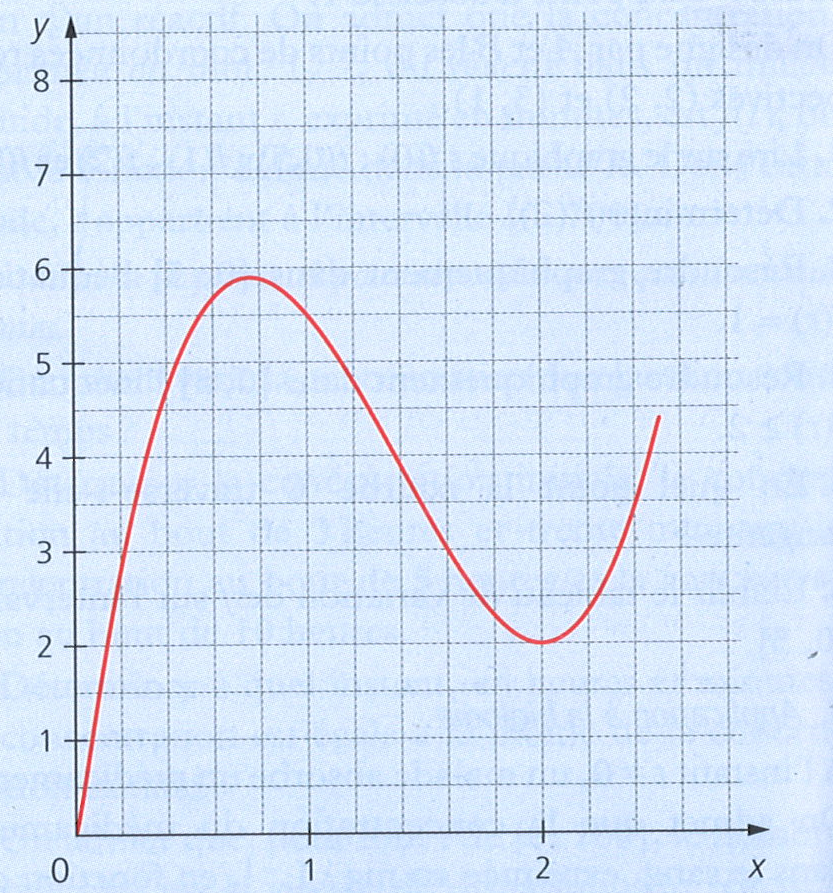
\includegraphics[scale=0.7]{img/courbe_31}
		
		\caption{Courbe $\mathcal{C}$}
		\label{fig:c}
	\end{figure}
%\end{center}

\label{LastPage}
	

\end{document}